\section{Opis implementacji}
Aplikacja została napisana przy użyciu języków programowania bazujących na maszynie wirtualnej javy:
\begin{enumerate}
  \item Kotlin - podstawowy język użtyty do implementacji (prawie 90\% projektu)
  \item Java 8 - język użyty do generowania statystyk wykonania algorytmów
  \item JavaFX - technologia zastosowana do stworzenia graficzego interfejsu użytkownika (wraz z CSS)
\end{enumerate}

Architektura aplikacji jest modułowa. Zostały wydzielone części odpowiedzialne za obliczenia matematyczne, implementacje algorytmów, zapis i odczyt plików CSV, generację statystyk, definicję modelu danych oraz moduł zawierający aplikację korzystająca z pozostałych pakietów (\hyperref[fig:arch]{rys.~\ref*{fig:arch}}).

\begin{figure}[h]
  \center
  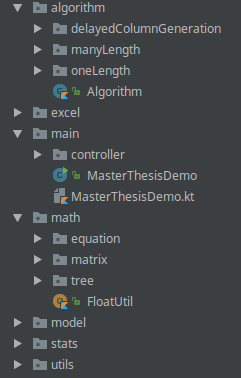
\includegraphics[scale=0.7]{../image/arch.png}
  \caption{Architektura aplikacji}
  \label{fig:arch}
\end{figure}

Architektura modułu odpowiedzialnego za implementację algorytmów posiada strukturę wzorca projektowego fasada. Klasy odpowiedzialne za konkretną implementację metody obliczenia rozkrojów rozszerzają klasę abstarkacyjną która definiuje wspólne funkcje oraz deklaruje metody które powinny zostać zdefiniowane w klasach potomnych. Główny moduł aplikacji wraz z modułem odpowiedizlanym za model danych tworzy implementację wzoraca Model-Widok-Kontroler (MVC). Klasa kontrolera zarządza widokiem stworzonym w języku FXML.

Rysunki \ref{fig:empty_win} oraz \ref{fig:fill_win} przedstawiają okno aplikacji, odpowiednio przed wypełnieniem danymi oraz po zakończeniu obliczeń.

\begin{figure}[h]
  \center
  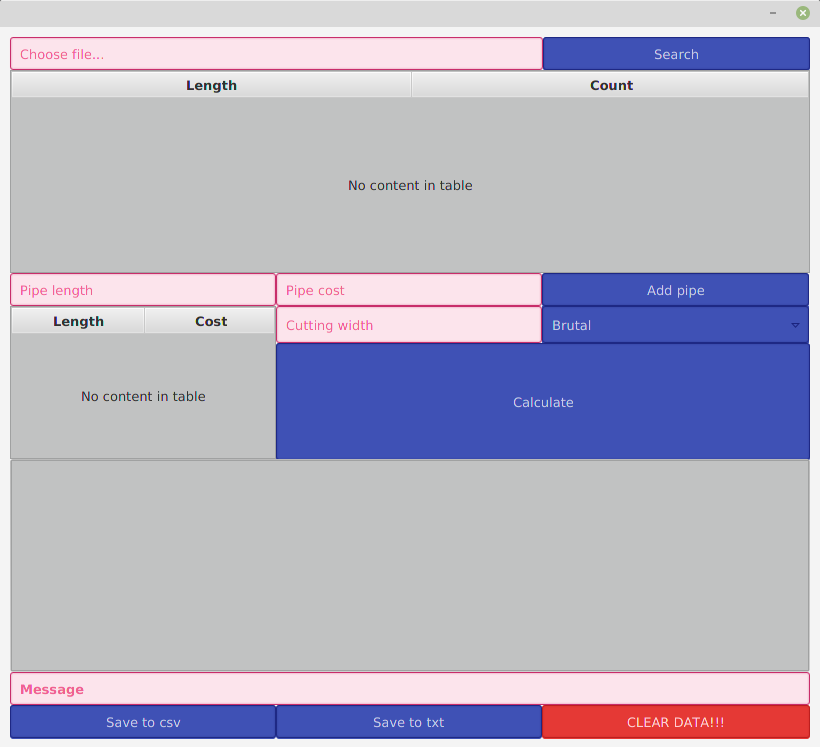
\includegraphics[scale=0.4]{../image/empty_win.png}
  \caption{Początkowe okno aplikacji}
  \label{fig:empty_win}
\end{figure}

\begin{figure}[h]
  \center
  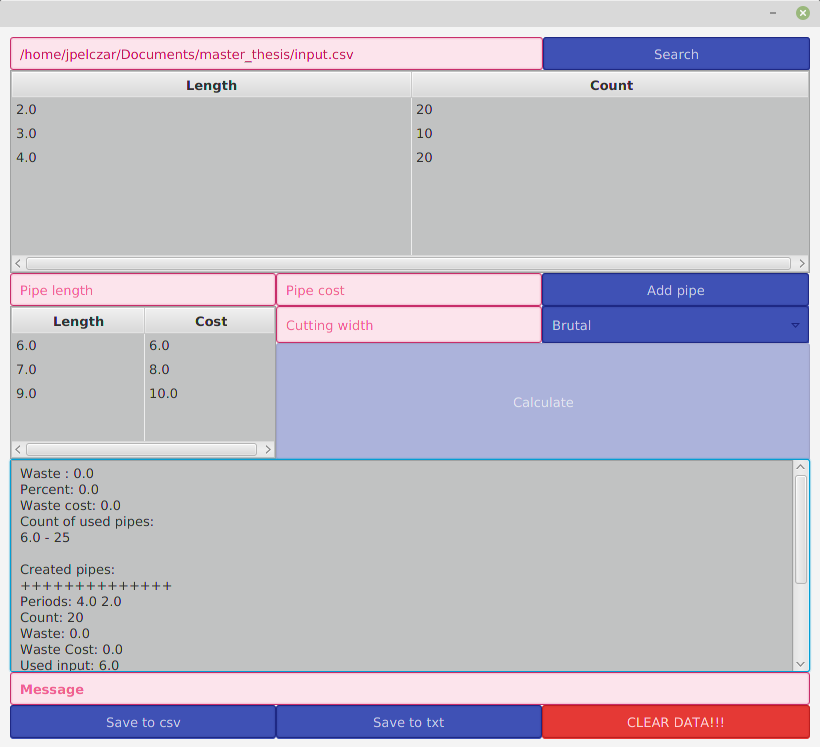
\includegraphics[scale=0.4]{../image/fill_win.png}
  \caption{Aplikacja po zakończonych obliczeniach}
  \label{fig:fill_win}
\end{figure}

Program posiada możliwość wczytania danych z pliku CSV, a następnie zapisanie danych wyjściowych również do pliku CSV lub TXT. Kolejnymi zaimplementowanymi funkcjonalnościami są:
\begin{enumerate}
  \item wyświetlenie danych wejściowych w oknie aplikacji
  \item wybór algorytmu rozkroju
  \item dodanie wielu długości podstawowych z różnym kosztem - domyślnie koszt jest równy długości.
  \item wyświetlenie długości podstawowych w oknie aplikacji
  \item dodanie szerkości cięcia dla metody brutalnej siły
  \item wyświetlenie wyniku w oknie aplikacji
\end{enumerate}

\subsection{Java}
Język programowania Java jest jezykiem obiektowym z elementami programowania funkcyjnego wprowadzonymi od wersji 8. Aplikacje stworzone w tej technologii mogą być stosowane w różnych systemach operacyjnych, gdyż programy napisane w języku Java są kompilowane do plików class które umieszczane są w skompresowanej paczce jar. Pliki class następnie są przetwarzane przez maszynę wirtualną Javy (JVM - Java Virtual Machine) do postaci bytocodu który jest wykonywany na urządzeniu. Istnieją implementacje JVM na większość używanych platform.

Tworzenie aplikacji w technologii Java jest możliwe poprzez użycie zestawu JDK (Java Development Kit). Uruchamianie tych aplikacji jest możliwe w środowisku JRE (Java Runtime Environment).
\subsection{Kotlin}
\subsection{JavaFX}
